\documentclass[alsotrans]{beamerswitch}
\usepackage{sdp}

\title{Стек}

\date{7--14 октомври 2019 г.}

\titlegraphicx{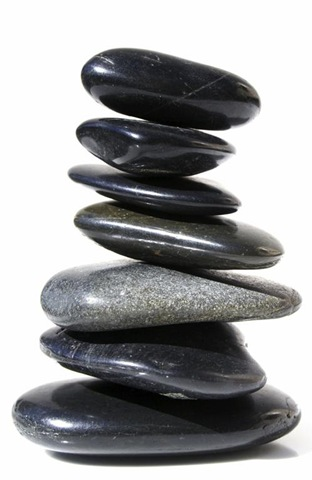
\includegraphics[height=0.25\textheight]{images/stack.jpg}\\
  \imageAttr{Stack of Rocks, Cattle Point, San Juan Island}{Ryan Harvey}{https://flic.kr/p/aojd1Q}{CC BY-SA 2.0}}

\begin{document}

\begin{frame}
  \titlepage
\end{frame}

\section{АТД стек}

\begin{frame}
  \frametitle{АТД: стек}

  Хомогенна линейна структура с организация ``последен влязъл --- пръв излязъл'' (LIFO)\\[1em]
  Операции\\[0.5em]
  \begin{itemize}
  \item \lst{create()} --- създаване на празен стек
  \item \lst{empty()} --- проверка за празнота на стек
  \item \lst{push(x)} --- включване на елемент на стек
  \item \lst{pop()} --- изключване на елемент от стек
  \item \lst{peek()} --- последен елемент на стека
  \end{itemize}
\end{frame}

\begin{frame}
  \frametitle{АТД: стек}

  Свойства на операциите\\[0.5em]
  \begin{itemize}
  \item \lst{create().empty()} = \lst{true}
  \item \lst{s.push(x).empty()} = \lst{false}
  \item \lst{create().peek()}, \lst{create().pop()} --- \alert{грешка}
  \item \lst{s.push(x).peek()} = \tt x
  \item \lst{s.push(x).pop()} = \tt s
  \end{itemize}
\end{frame}

\begin{frame}
  \frametitle{Последователно представяне на стек}

  \begin{center}
    \begin{tikzpicture}
      % масивът
      \matrix (a) [widearray] {
        a_0 \& a_1 \& a_2 \& \ldots \& |(an)| a_n \& |(an+1)| \alt<1>{}{a_{n+1}} \&\&\&\&\\
      };

      % индекс на върха на стека
      \pointerto[visible on=<{1,3}>]{an}{\tt{top}}{below}

      % индекс на върха на стека след добавяне на елемент
      \pointerto[visible on=<2>]{an+1}{\tt{top}}{below}

    \end{tikzpicture}
  \end{center}

  \begin{itemize}
  \item<2-> включване на елемент (push)
  \item<3-> изключване на елемент (pop)
  \end{itemize}
\end{frame}

\begin{frame}<1-6>[fragile]
  \frametitle{Свързано представяне на стек}

  Представяме стека като ``верига'' от двойни кутии

  \begin{center}
    \scriptsize
    \begin{tikzpicture}
      % веригата
      \doublecell{an}{a_n}
      \nextdoublecell{an-1}{a_{n-1}}{an}

      \node (dots) [right=2ex of an-1] {...\hspace{2ex}};
      \draw[pointer] (an-1next.center) to (dots.west);

      \doublecell[right=2ex of dots]{a1}{a_1}
      \draw[pointer] (dots.east) to (a1data);

      \nextdoublecell{a0}{a_0}{a1}
      \nullptr{a0next}

      % указател към върха
      \begin{scope}[visible on=<{1,4-}>]
        \pointerto{an.south}{\tt{top}}{below}
      \end{scope}

      % новата клетка
      \begin{scope}[visible on=<2-5>]
        \doublecell[left=4ex of an]{an+1}{a_{n+1}}
        \draw[pointer] (an+1next.center) to (an);
      \end{scope}

      % преместване на указателя към върха
      \begin{scope}[visible on=<2-3>]
        \pointerto{an+1.south}{\tt{top}}{below}
      \end{scope}

      % нов указател
      \begin{scope}[visible on=<3-5>]
        \pointerto{an+1data.south}{\tt{p}}{below left}
      \end{scope}

      % изтриване на новата клетка
      \draw (an+1) node[cross,visible on=<5>] {};

    \end{tikzpicture}
  \end{center}

\begin{lstlisting}
struct StackElement {
	int data;
	StackElement* next;
};
\end{lstlisting}

  \begin{itemize}
  \item<2-> включване на елемент (push)
  \item<3-> изключване на елемент (pop)
  \end{itemize}

\end{frame}

\section{Приложения на стек}

\subsection{Пресмятане на израз}

\begin{frame}
  \frametitle{Обратен полски запис}

  % TODO: анимация на обхожданията
  \begin{columns}[t,onlytextwidth]
    \begin{column}{.6\textwidth}
      \begin{itemize}
      \item инфиксен запис:\\
        \lst{(1+2)*(3-4/5)}
      \item префиксен (полски) запис:\\
        \lst{*+12-3/45}
      \item постфиксен (обратен полски) запис\\
        \lst{12+345/-*}
      \end{itemize}
    \end{column}

    \begin{column}{0.4\textwidth}
      \begin{center}
        \begin{forest} for tree={circle,draw,fill=diagramblue}
          [\tt* [\tt+ [\tt1] [\tt2]] [\tt- [\tt3] [\tt/ [\tt4] [\tt5]]]]
        \end{forest}
      \end{center}
    \end{column}
  \end{columns}
\end{frame}

\begin{frame}
  \frametitle{Пресмятане на израз в обратен полски запис}

  \begin{center}
    \begin{tikzpicture}[scale=1.3]
      \filldraw[fill=diagramblue,draw=black] (0, 0) -- (4, 0) -- (4, -2) -- (2, -2) -- (2, -4) -- (0, -4) -- (0, 0);
      \node[align=center] at (3, -1) {обратен\\полски\\запис};
      \node at (1, -3) {резултати};
    \end{tikzpicture}
  \end{center}
\end{frame}

\begin{frame}
  \frametitle{Алгоритъм за пресмятане на обратен полски запис}
  За всеки пореден символ \tt c от израза в обратен полски запис:\pause
  \begin{itemize}[<+->]
  \item Ако \tt c е цифра, добавяме стойността ѝ в стека за резултати
  \item Ако \tt c е (двуместна) операция:
    \begin{itemize}
    \item изваждаме най-горните два елемента от стека
    \item прилагаме операцията над тях
    \item добавяме резултата в стека
    \end{itemize}
  \end{itemize}
  \onslide<+->
  В стека остава единствен елемент: крайният резултат.
\end{frame}

\begin{frame}<trans:0>
  \frametitle{Пример: Пресмятане на израз в обратен полски запис}

  \begin{center}
    \begin{tikzpicture}[scale=1.3]
      \filldraw[fill=diagramblue,draw=black] (0, 0) -- (4, 0) -- (4, -2) -- (2, -2) -- (2, -4) -- (0, -4) -- (0, 0);
      \node[anchor=base east,align=right] at (4, -1.1) {%
        \tt{%
          \only<-+>1%
          \only<-+>2%
          \only<-+>+%
          \only<-+>3%
          \only<-+>4%
          \only<-+>5%
          \only<-+>/%
          \only<-+>-%
          \only<-+>*%
        }};
      \node[anchor=south,align=center] at (1, -4) {%
        \only<10>{\\\tt{6.6}}%
        \only<9>{\\\tt{2.2}}%
        \only<8>{\\\tt{0.8}}%
        \only<7>{\\\tt 5}%
        \only<6-7>{\\\tt 4}%
        \only<5-8>{\\\tt 3}%
        \only<4-9>{\\\tt 3}%
        \only<3>{\\\tt 2}%
        \only<2-3>{\\\tt 1}%
      };
    \end{tikzpicture}
  \end{center}
\end{frame}

\begin{frame}
  \frametitle{Преобразуване в обратен полски запис}

  \begin{center}
    \begin{tikzpicture}[scale=1.3]
      \filldraw[fill=diagramblue,draw=black]
      (-2, 0) -- (4, 0) -- (4, -2) -- (2, -2) -- (2, -4) -- (0, -4) -- (0, -2) -- (-2, -2) -- (-2, 0);
      \node[align=center] at (3, -1) {инфиксен\\запис};
      \node[align=center] at (-1, -1) {обратен\\полски\\запис};
      \node[align=center] at (1, -3) {операции};
    \end{tikzpicture}
  \end{center}
\end{frame}

\begin{frame}<1-6| trans:1>[label=shunting]
  \frametitle{Алгоритъм на разпределителната гара (shunting yard)}
  \begin{overlayarea}{\textwidth}{.8\textheight}
    За преобразуване от инфиксен в обратен полски запис, за всеки пореден символ \tt c:\\\pause
    \begin{itemize}[<+->]
    \item Ако \tt c е цифра, прехвърляме я в \alt<-9| trans:1-2>{\alert<9| trans:0>{крайния резултат}}{стека с резултати}
    \item Ако \tt c е отваряща скоба, поставяме я в стека с операции
    \item Ако \tt c е операция\alt<-7| trans:1>{\alert<7| trans:0>{, поставяме я в стека с операции}}:
      \only<8-| trans:2-3>{%
        \begin{itemize}
        \item изваждаме от стека \alt<-11| trans:1-2>{\alert<11| trans:0>{и записваме в резултата}}{и прилагаме} всички операции с приоритет по-висок или равен на \tt c
        \item поставяме \tt c в стека
        \end{itemize}
        }%
    \item Ако \tt c е затваряща скоба, последователно изваждаме от стека \alt<-11| trans:1-2>{\alert<11| trans:0>{и записваме в резултата}}{и прилагаме} всички операции до достигане на отваряща скоба
    \end{itemize}
    \onslide<6->
    След приключване на входния низ, последователно изваждаме от стека и \alt<-11| trans:1-2>{\alert<11| trans:0>{и записваме в резултата}}{и прилагаме} всички останали операции.

    \onslide<12-| trans:3>
    \alert<trans:0>{Крайният резултат е единственият елемент в стека с резултати}.
  \end{overlayarea}
\end{frame}

\begin{frame}<trans:0>
  \frametitle{Пример: Преобразуване в обратен полски запис}

  \begin{center}
    \begin{tikzpicture}[scale=1.3]
      \filldraw[fill=diagramblue,draw=black]
      (-2, 0) -- (4, 0) -- (4, -2) -- (2, -2) -- (2, -4) -- (0, -4) -- (0, -2) -- (-2, -2) -- (-2, 0);
      \node[anchor=west,align=left] at (-2, -1) {%
        \tt{%
          \only<3->1%
          \only<5->2%
          \only<8->+%
          \only<12->3%
          \only<14->4%
          \only<16->5%
          \only<19->/%
          \only<20->-%
          \only<22->*%
        }};
      \node[anchor=east,align=right] at (4, -1) {%
        \tt{%
          \only<-1>(%
          \only<-2>1%
          \only<-3>+%
          \only<-4>2%
          \only<-5>)%
          \only<-9>*%
          \only<-10>(%
          \only<-11>3%
          \only<-12>-%
          \only<-13>4%
          \only<-14>/%
          \only<-15>5%
          \only<-16>)%
        }};
      \node[anchor=south,align=center] at (1, -4) {%
        \only<17>{\\\tt)}%
        \only<15-18>{\\\tt/}%
        \only<13-19>{\\\tt-}%
        \only<11-20>{\\\tt(}%
        \only<10-21>{\\\tt*}%
        \only<6>{\\\tt)}%
        \only<4-7>{\\\tt+}%
        \only<2-8>{\\\tt(}%
      };
    \end{tikzpicture}
  \end{center}
\end{frame}

\begin{frame}
  \frametitle{Приоритети на операциите}
  Какъв е обратния полски запис на израза \tt{(1+2)*(3/4-5)}?
  \begin{itemize}[<+->]
  \item Ако следваме алгоритъма, описан по-рано, резултатът би трябвало да е \tt{12+345-/*}\ldots
  \item \ldots \alert{но резултатът от този израз е \tt{-9}, а не \tt{-12.75}!}
  \item На обратния полски запис \tt{12+345-/*} съответсва инфиксен запис \tt{(1+2)*(3/(4-5))}!
  \item \alert{Не сме взели предвид по-високия приоритет на операцията \tt/}
  \item Правилният обратен полски запис на \tt{(1+2)*(3/4-5)} е \tt{12+34/5-*}.
  \item \alert{Необходимо е да променим алгоритъма, така че да взема предвид приоритета на операциите!}
  \end{itemize}
\end{frame}

\againframe<7-8| trans:2>{shunting}

\begin{frame}<trans:0>
  \frametitle{Пример 2: Преобразуване в обратен полски запис}

  \begin{center}
    \begin{tikzpicture}[scale=1.3]
      \filldraw[fill=diagramblue,draw=black]
      (-2, 0) -- (4, 0) -- (4, -2) -- (2, -2) -- (2, -4) -- (0, -4) -- (0, -2) -- (-2, -2) -- (-2, 0);
      \node[anchor=west,align=left] at (-2, -1) {%
        \tt{%
          \only<3->1%
          \only<5->2%
          \only<8->+%
          \only<12->3%
          \only<14->4%
          \only<15->/%
          \only<16->5%
          \only<19->-%
          \only<21->*%
        }};
      \node[anchor=east,align=right] at (4, -1) {%
        \tt{%
          \only<-1>(%
          \only<-2>1%
          \only<-3>+%
          \only<-4>2%
          \only<-5>)%
          \only<-9>*%
          \only<-10>(%
          \only<-11>3%
          \only<-12>/%
          \only<-13>4%
          \only<-14>-%
          \only<-15>5%
          \only<-16>)%
        }};
      \node[anchor=south,align=center] at (1, -4) {%
        \only<17>{\\\tt)}%
        \only<15-18>{\\\tt-}%
        \only<13-14>{\\\tt/}%
        \only<11-19>{\\\tt(}%
        \only<10-20>{\\\tt*}%
        \only<6>{\\\tt)}%
        \only<4-7>{\\\tt+}%
        \only<2-8>{\\\tt(}%
      };
    \end{tikzpicture}
  \end{center}
\end{frame}

\begin{frame}
  \frametitle{Директно пресмятане на израз}

  Ако комбинираме двата алгоритъма, можем да пресмятаме инфиксен израз директно, без използването на обратен полски запис:
  \begin{center}
    \begin{tikzpicture}[scale=1.3]
      \filldraw[fill=diagramblue,draw=black]
      (-4, 0)  -- (4, 0)   -- (4, -2) -- (2, -2) -- (2, -4) -- (0, -4) -- (0, -2) -- (-2, -2) --
      (-2, -4) -- (-4, -4) -- (-4, 0);
      \node[align=center] at (3, -1) {инфиксен\\запис};
      \node at (-3, -3) {резултати};
      \node at (1, -3) {операции};
    \end{tikzpicture}
  \end{center}
\end{frame}

\againframe<9-13| trans:3>{shunting}

\begin{frame}<trans:0>
  \frametitle{Пример: Директно пресмятане на израз}

  \begin{center}
    \begin{tikzpicture}[scale=1.3]
      \filldraw[fill=diagramblue,draw=black]
      (-4, 0)  -- (4, 0)   -- (4, -2) -- (2, -2) -- (2, -4) -- (0, -4) -- (0, -2) -- (-2, -2) --
      (-2, -4) -- (-4, -4) -- (-4, 0);
      \node[anchor=base east,align=right] at (4, -1) {%
        \tt{%
          \only<-1>(%
          \only<-2>1%
          \only<-3>+%
          \only<-4>2%
          \only<-5>)%
          \only<-9>*%
          \only<-10>(%
          \only<-11>3%
          \only<-12>-%
          \only<-13>4%
          \only<-14>/%
          \only<-15>5%
          \only<-16>)%
        }};
      \node[anchor=south,align=center] at (-3, -4) {%
        \only<22>{\\\tt{6.6}}%
        \only<20-21>{\\\tt{2.2}}%
        \only<19>{\\\tt{0.8}}%
        \only<16-18>{\\\tt5}%
        \only<14-18>{\\\tt4}%
        \only<12-19>{\\\tt3}%
        \only<8-21>{\\\tt3}%
        \only<5-7>{\\\tt2}%
        \only<3-7>{\\\tt1}%
      };
      \node[anchor=south,align=center] at (1, -4) {%
        \only<17>{\\\tt)}%
        \only<15-18>{\\\tt/}%
        \only<13-19>{\\\tt-}%
        \only<11-20>{\\\tt(}%
        \only<10-21>{\\\tt*}%
        \only<6>{\\\tt)}%
        \only<4-7>{\\\tt+}%
        \only<2-8>{\\\tt(}%
      };
    \end{tikzpicture}
  \end{center}
\end{frame}

\begin{frame}<trans:0>
  \frametitle{Пример 2: Директно пресмятане на израз}

  \begin{center}
    \begin{tikzpicture}[scale=1.3]
      \filldraw[fill=diagramblue,draw=black]
      (-4, 0)  -- (4, 0)   -- (4, -2) -- (2, -2) -- (2, -4) -- (0, -4) -- (0, -2) -- (-2, -2) --
      (-2, -4) -- (-4, -4) -- (-4, 0);
      \node[anchor=base east,align=right] at (4, -1) {%
        \tt{%
          \only<-1>(%
          \only<-2>1%
          \only<-3>+%
          \only<-4>2%
          \only<-5>)%
          \only<-9>*%
          \only<-10>(%
          \only<-11>3%
          \only<-12>/%
          \only<-13>4%
          \only<-16>{\alert<15>-}%
          \only<-17>5%
          \only<-18>)%
        }};
      \node[anchor=south,align=center] at (-3, -4) {%
        \only<23>{\\\tt{-12.75}}%
        \only<21-22>{\\\tt{-4.25}}%
        \only<18-20>{\\\tt5}%
        \only<16-20>{\\\tt{0.75}}%
        \only<14-15>{\\\tt4}%
        \only<12-15>{\\\tt3}%
        \only<8-22>{\\\tt3}%
        \only<5-7>{\\\tt2}%
        \only<3-7>{\\\tt1}%
      };
      \node[anchor=south,align=center] at (1, -4) {%
        \only<19>{\\\tt)}%
        \only<17-20>{\\\tt-}%
        \only<13-15>{\\\alert<15>{\tt/}}%
        \only<11-21>{\\\tt(}%
        \only<10-22>{\\\tt*}%
        \only<6>{\\\tt)}%
        \only<4-7>{\\\tt+}%
        \only<2-8>{\\\tt(}%
      };
    \end{tikzpicture}
  \end{center}
\end{frame}

\begin{frame}
  \frametitle{Поточна обработка на израз}
  Комбинирането на двата алгоритъма може да се получи по естествен начин при използване на \alert{поточна обработка}:\pause
  \begin{itemize}[<+->]
  \item Алгоритъм 1 (разпределителна гара)
    \begin{itemize}
    \item консумира поток от символи на израз в инфиксен запис
    \item произвежда поток от символи на израз в обратен полски запис
    \end{itemize}
  \item Алгоритъм 2 (пресмятане на обратен полски запис):
    \begin{itemize}
    \item консумира поток от символи на израз в обратен полски запис
    \item произвежда поток от числа (върховете на стека с резултати)
    \end{itemize}
  \item Алгоритъм 3 = Алгоритъм 1 | Алгоритъм 2:
    \begin{itemize}
    \item консумира поток от символи на израз в инфиксен запис
    \item произвежда поток от числа (върховете на стека с резултати)
    \end{itemize}
  \item Предимства на поточната обработка:
    \begin{itemize}
    \item позволява гъвкаво комбиниране на различни алгоритми
    \item показва частични резултати
    \item може да работи потенциално безкрайно
    \end{itemize}
  \end{itemize}
\end{frame}

\subsection{Симулиране на рекурсия}

\begin{frame}
  \frametitle{Симулиране на рекурсия}

  \begin{itemize}
  \item Стекова рамка
    \begin{itemize}
    \item при извикване на функция
    \item при рекурсия
    \end{itemize}
  \item Стек вместо стекова рамка
  \item Пример: ход на коня
  \end{itemize}
\end{frame}

\begin{frame}
  \frametitle{Пример: ход на коня}

  \begin{columns}[T,onlytextwidth]
    \begin{column}{.5\textwidth}
      \setboardfontsize{2em}
      \begin{tikzpicture}
        \matrix[chessboard=2em] {%
          \bks1\&\&\bks9\&\\
          \bks{10,11}\&\&\bks2\&\bks5\\
          \bks3\&\safetemporal6{}\bk{\alt<8>\bk\wk}\&\&\\
          \&\&\bks4\&\safetemporal7{}\bk\rk\\
        };
      \end{tikzpicture}
    \end{column}

    \begin{column}{.5\textwidth}
      \begin{tabular}{|c|cc}
        \cline{1-1}
        \\\cline{1-1}
        \\\cline{1-1}\onslide<10->{(1,0)}
        \\\cline{1-1}\onslide<7->{\safetemporal8{(3,3)}{}{(0,2)}}
        \\\cline{1-1}\onslide<6->{(2,1)}&\gc{11-}{(0,1)}
        \\\cline{1-1}\onslide<5->{(1,3)}&\gc{11-}{(1,1)}
        \\\cline{1-1}\onslide<4->{(3,2)}&\gc{11-}{(0,1)}
        \\\cline{1-1}\onslide<3->{(2,0)}&\gc{11-}{(3,1)}&\gc{11-}{(3,3)}
        \\\cline{1-1}\onslide<2->{(1,2)}&\gc{11-}{(2,1)}
        \\\cline{1-1}\onslide<1->{(0,0)}
        \\\cline{1-1}
      \end{tabular}
    \end{column}
  \end{columns}
\end{frame}

\section{STL}

\begin{frame}
  \frametitle{\lst{std::stack<T>}}

  \begin{itemize}
  \item \lst{stack()} --- създаване на празен стек
  \item \lst{empty()} --- проверка за празнота на стек
  \item \lst{push(x)} --- включване на елемент на стек
  \item \lst{pop()} --- изключване на елемент от стек
  \item \lst{top()} --- последен елемент на стека
  \item \lst{size()} --- дължина на стека
  \item \lst{==,!=,<,>,<=,>=} --- лексикорафско сравнение на два стека
  \end{itemize}
\end{frame}

\end{document}
